\subsection{Dataset}
We utilized the MinneApple dataset, ...

The average object categories and numbers of objects in each image for these datasets are summarised in Tab.~\ref{tab:categories}.  

\begin{table}[htb]
\centering
\caption{Number of categories contained in each image and the number of instances of each category of the four datasets~\citep{Haeni2020}}
\label{tab:categories}
\resizebox{\textwidth}{!}{%
\begin{tabular}{@{}p{4.5cm}<{\centering} p{2.5cm}<{\centering} p{2.5cm}<{\centering} p{2.5cm}<{\centering} p{3cm}<{\centering}@{}}
\toprule
                       & MinneApple & COCO & ImageNet & PASCAL VOC \\ \midrule
Number of categories   & 1.5        & 3.5  & $\le 2$  & $\le 2$    \\
Instances per category & 41.2       & 7.7  & $\le 3$  & $\le 3$    \\ \bottomrule
\end{tabular}%
}
\end{table}


\subsection{Data Quality}
We ... Most of the images in the counting dataset are ... and have a resolution ... (Fig.~\ref{fig:counting dataset images}).

\begin{figure}[htb]
    \centering
    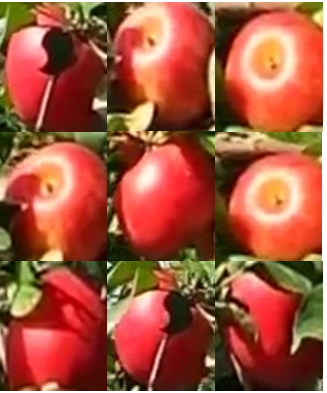
\includegraphics[width=0.3\textwidth]{images/counting_dataset.png}
    \caption{Caption~\citep{Haeni2020}}
    \label{fig:counting dataset images}
\end{figure}




